%%%%%%%%%%%%%%%%%%%%%%%%%%%%%%%%%%%%%%%%%%%%%%%%%%%%%%%%%%%%%%%%%%%%%%
% Universidade Federal de Santa Catarina             
% Biblioteca Universitária                     
%----------------------------------------------------------------------
% Exemplo de utiliza\c{C}ão da documentclass ufscThesis
%----------------------------------------------------------------------
% (c)2013 Roberto Simoni (roberto.emc@gmail.com)
%         Carlos R Rocha (cticarlo@gmail.com)
%         Rafael M Casali (rafaelmcasali@yahoo.com.br)
%%%%%%%%%%%%%%%%%%%%%%%%%%%%%%%%%%%%%%%%%%%%%%%%%%%%%%%%%%%%%%%%%%%%%%%
\documentclass{ufscThesis} % Definicao do documentclass ufscThesis	

%----------------------------------------------------------------------
% Pacotes usados especificamente neste documento
\usepackage{graphicx} % Possibilita o uso de figuras e gráficos
\usepackage{color}    % Possibilita o uso de cores no documento
\usepackage{listings}
%\usepackage{amsmath}
%----------------------------------------------------------------------
% Comandos criados pelo usuário
\newcommand{\afazer}[1]{{\color{red}{#1}}} % Para destacar uma parte a ser trabalhada

%----------------------------------------------------------------------
% Identificadores do trabalho
% Usados para preencher os elementos pré-textuais
\instituicao[a]{Universidade Federal de Santa Catarina} % Opcional
\departamento[a]{Departamento de Inform\'atica e Estat\'istica}
\curso[o]{Bacharel em Ci\^encias da Computa\c{c}\~ao}
\documento[a]{Trabalho de conclus\~ao de curso} % [o] para disserta\c{C}ão [a] para tese
\titulo{Implementa\c{c}\~ao do protocolo CoAP para o monitoramento em redes de sensores sem fio}
\autor{Rafael de Lucena Valle}
\local{Florian\'opolis} % Opcional (Florianópolis é o padrão)
\data{15}{julho}{2013}
\orientador[Orientador]{Prof. Dr. Ant\^onio Augusto Fr\"ohlich}
\coorientador[Coorientador]{Prof. M.Sc. Arliones Hoeller Jr}
\coordenador[Coordenador]{Prof. Dr. Roberto Cislaghi}

\numerodemembrosnabanca{4} % Isso decide se haverá uma folha adicional
\orientadornabanca{sim} % Se faz parte da banca definir como sim
\coorientadornabanca{sim} % Se faz parte da banca definir como sim
\bancaMembroA{Prof. M.Sc. Arliones Hoeller Jr} %Nome do presidente da banca
\bancaMembroB{Prof. Dr. Ant\^onio Augusto Fr\"ohlich} % Nome do membro da Banca
\bancaMembroC{Prof. Dr. Eng. Rafael Luiz Cancian} % Nome do membro da Banca
\bancaMembroD{Prof. Dr. Frank Siqueira} % Nome do membro da Banca

\agradecimento{Inserir os agradecimentos aos colaboradores \'a execu\c{c}\~ao do trabalho.}

\textoResumo {Redes de sensores s\~ao utilizadas para a capta\c{c}\~ao, processamento de informa\c{c}\~ao e atua\c{c}\~ao sobre um ambiente, tornando-as importantes para controle, telemetria e rastreamento de sistemas. Os n\'os das redes geralmente s\~ao computadores e r\'adios simplificados, que possuem restri\c{c}\~oes de mem\'oria, processamento, energia e comunica\c{c}\~ao, mas um custo relativamente baixo de equipamentos, tornando interessante a implanta\c{c}\~ao destes sistemas. O protocolo HTTP foi desenvolvido pensado em computadores de prop\'osito geral, onde essas restri\c{c}\~oes n\~ao existem. Um protocolo leve como CoAP pode tornar viável a cria\c{c}\~ao de aplica\c{c}\~oes web em redes de sensores sem fio por um baixo custo.

\'E proposto uma infraestrutura de comunica\c{c}\~ao entre redes de sensores sem fio e a Internet, utilizando protocolos leves entre os n\'os sensores e um gateway GPRS para \'areas sem acesso \'a WIFI, aproveitando a vasta abrang\^encia da tecnologia de telefonia. Com a Utiliza\c{c}\~ao do CoAP \'e esperado uma redu\c{c}\~ao de consumo de energia e mem\'oria, em rela\c{c}\~ao a outros protocolos de aplica\c{c}\~ao existentes.}

\palavrasChave{ internetworking wireless sensor networks IPv6 6LoWPAN GPRS CoAP }

%----------------------------------------------------------------------
% Início do documento                                
\begin{document}
%--------------------------------------------------------
% Elementos pré-textuais
\capa
\folhaderosto%[comficha] % Se nao quiser imprimir a ficha, é só não usar o parâmetro
\folhaaprovacao
%\paginadedicatoria
\paginaagradecimento
%\paginaepigrafe

\paginaresumo
%\paginaabstract
%\pretextuais % Substitui todos os elementos pre-textuais acima
\listadefiguras % as listas dependem da necessidade do usuário
%\listadetabelas 
\listadeabreviaturas
%\listadesimbolos
\sumario
%--------------------------------------------------------
% Elementos textuais

\chapter{Introdu\c{c}\~ao}
Redes de sensores e atuadores s\~ao utilizadas para a capta\c{c}\~ao, processamento de informa\c{c}\~ao e atua\c{c}\~ao sobre um ambiente, tornando-as importantes em aplica\c{c}\~oes de controle, telemetria e rastreamento de sistemas.

N\'os que participam destas redes geralmente s\~ao compostos por computadores e r\'adios simplificados, que possuem restri\c{c}\~oes de mem\'oria, processamento, energia e capacidade de comunica\c{c}\~ao, mas um custo relativamente baixo de equipamentos.

O maior consumo de energia neste tipo de aplica\c{c}\~ao \'e do r\'adio, portanto o desafio dos algoritmos de comunica\c{c}\~ao nesta \'area \'e manter os r\'adios ligados o m\'inimo de tempo poss\'ivel sem comprometer a conectividade do n\'o.

\section{Objetivos}
O objetivo geral desse trabalho \'e descrever e implementar webservices em uma rede sensores sem fio que far\~ao a aquisi\c{c}\~ao dos dados do ambiente e disponibilizar\~ao as informa\c{c}\~oes captadas na Internet.

\subsection{Objetivos Espec\'ificos}
Este trabalho realizar\'a o desenvolvimento de aplica\c{c}\~oes web e software de sistema para fazer a ponte entre a rede de sensores e a Internet. O Sistema operacional utilizado ser\'a o EPOS, que possui uma implementa\c{c}\~ao de pilha UDP/IP. A aplica\c{c}\~ao integradora GPRS/802.15.4 ir\'a executar na plataforma EposMoteII utilizando uma extens\~ao GPRS.

A comunica\c{c}\~ao entre os n\'os da rede ser\'a feita atrav\'es do protocolo de aplica\c{c}\~ao CoAP, um protocolo espec\'ifico para redes de sensores sem fio. Ser\'a utilizado um porte de uma implementa\c{c}\~ao livre do protocolo CoAP.

Sendo assim, os objetivos espec\'ificos s\~ao:

\begin{enumerate}
    \item{Portar o protocolo CoAP para o EPOS;}
    \item{Implementar uma aplica\c{c}\~ao para redes de sensores sem fio;}
    \item{Desenvolver a aplica\c{c}\~ao gateway GPRS/802.15.4.}
    \item{Desenvolver uma aplica\c{c}\~ao web para visualiza\c{c}\~ao da informa\c{c}\~ao;}
    \item{Avaliar a soluc\c{c}\~ao desenvolvida.}
\end{enumerate}

\section{Justificativa}

Os mecanismos de confiabilidade na transmiss\~ao de dados, t\'ecnicas para se manter uma conex\~ao do TCP e rearranjos que s\~ao feitos para garantir a ordem das mensagens recebidas n\~ao s\~ao adequados para um dispositivos com suprimento limitado de energia, como uma bateria ou uma placa fotovolt\'aica. Estas t\'ecnicas fazem que os transmissores fiquem ligados por mais tempo, para manter a conex\~ao ou at\'e mesmo para reenvio de mensagens.

O maior consumo de energia de um n\'o sensor \'e no envio e recebimento de dados, quando mantem seu transmissor ligado. Al\'em disso quem recebe a mensagem precisa mont\'a-la e tratar as partes corrompidas, podendo gerar retransmiss\~oes.

Por sua vez o protocolo do UDP, n\~ao mant\'em conex\~ao, dados s\~ao recebidos fora de ordem e o envio \'e feito de uma mensagem por vez. Isto implica tamb\'em na redu\c{c}\~ao do tamanho do cabe\c{c}alho do pacote.

Estas caracter\'isticas demostram uma alternativa interessante para estes equipamentos limitados. Testes feitos em implementa\c{c}\~oes de sistemas operacionais similares ao EPOS, como Contiki e TinyOS, utilizando o protocolo CoAP demonstram redu\c{c}\~ao no consumo de energia e mem\'oria em rela\c{c}\~ao ao HTTP \cite{transportApp}.

A falta de padroniza\c{c}\~ao dos protocolos afeta o desenvolvimento de uma rede p\'ublica ub\'iqua de uma cidade inteligente, por exemplo. Grande parte das solu\c{c}\~oes utiliza protocolos propriet\'arios que se comunicacam apenas com os produtos de um mesmo fabricante.

O protocolo HTTP foi desenvolvido para comunica\c{c}\~ao de computadores de prop\'osito geral, onde as restri\c{c}\~oes citadas n\~ao s\~ao comuns. Em rela\c{c}\~ao ao tamanho, o pacote HTTP \'e um problema para redes 802.15.4, j\'a que estas redes possuem uma restri\c{c}\~ao de 128 bytes em sua PDU. O protocolo TCP precisa transmitir mensagens adicionais para manter uma conex\~ao, outra caracter\'istica que n\~ao \'e interessante para RSSF.

Um protocolo leve como CoAP pode tornar vi\'avel a cria\c{c}\~ao de aplica\-\c{c}\~oes web em redes de sensores sem fio por um baixo custo. Neste trabalho \'e proposto uma infraestrutura de comunica\c{c}\~ao entre redes de sensores sem fio e a Internet, utilizando protocolos leves entre os n\'os sensores e um gateway GPRS para \'areas sem acesso \`a WIFI, aproveitando a vasta abrang\^encia da tecnologia de telefonia. Com a utiliza\c{c}\~ao do CoAP \'e esperado uma redu\c{c}\~ao de consumo de energia e mem\'oria, em rela\c{c}\~ao a outros protocolos de aplica\c{c}\~ao existentes.

Em lugares aonde n\~ao existe o acesso a rede cabeada ou sem fio, como lugares afastados, na \'area rural, por exemplo a distribui\c{c}\~ao da informa\c{c}\~ao para Internet ser\'a feita atrav\'es de um gateway.

O gateway ser\'a composto por um EposMoteII e um m\'odulo GPRS, respons\'avel por fazer a ponte entre a rede de sensores e a Internet. Atualmente o padr\~ao GPRS oferece a maior cobertura dentre as tecnologias de transmiss\~ao de telefonia no Brasil, atingindo cerca de 5477 munic\'ipios.\cite{coberturaGPRS}


\section{Metodologia}

Ser\'a feito um levantamento dos componentes de software e hardware necess\'arios para o desenvolvimento do gateway 802.15.4/GPRS. Neste caso utilizando o mote EPOSMote II e um m\'odulo GPRS, que ser\'a desenvolvido em paralelo a implementa\c{c}\~ao do protocolo de aplica\c{c}\~ao CoAP no sistema operacional EPOS.

Durante o desenvolvimento do protocolo, testes ser\~ao executados para verificar o correto comportamento e diminuir a depura\c{c}\~ao em hardware, que geralmente leva mais tempo.

Nos testes de integra\c{c}\~ao do gateway, ser\'a utilizada uma placa de desenvolvimento em conjunto com um m\'odulo M95 da Quectel disponibilizada pelo LISHA. Ser\~ao realizads testes de envio de mensagens em diversos protocolos, inclusive testes com comandos propriet\'arios adicionais do modem.

Para testes de integra\c{c}\~ao, as aplica\c{c}\~oes ser\~ao executadas na plataforma de sensores sem fio EPOS Mote II utilizando o EPOS com o CoAP desenvolvido.


\chapter{Desenvolvimento}
Este trabalho implementa uma biblioteca que utiliza a camada UDP do EPOS para dar suporte ao protocolo CoAP, uma aplica\c{c}\~ao gateway GPRS/802.14.5 utilizando o EPOS e um componente de hardware GPRS que ser\'a acoplado ao EposMoteII.

Para isto foram realizados diversos estudos durante o desenvolvimento do protocolo, pesquisas para escolher um m\'odulo GPRS adequado a tarefa. Al\'em disso testes de valida\c{c}\~ao dos sistemas de software e valida\c{c}\~ao do m\'odulo GPRS, levantamento de requisitos para porte de uma biblioteca CoAP para o EPOS (libCoap, libCantCoap, microCoap, entre outras) e EPOSMoteII.

Porte da biblioteca para o EPOS. Utilizando testes para validar o funcionamento entre diferentes arquiteturas e compiladores. A execu\c{c}\~ao dos testes foi feita no Qemu.

Implementa\c{c}\~ao dos mecanismos de transmiss\~ao para mensagens confirm\'aveis e n\~ao-confim\'aveis, requisi\c{c}\~ao e resposta.

A aplica\c{c}\~ao que ser\'a respons\'avel pelo roteamento de mensagens para Internet utiliza a tecnologia GPRS, provida por um m\'odulo GSM/GPRS da Quectel o M95.

\section{Levantamento de Requisitos}
Infraestrutura flex\'ivel para a contru\c{c}\~ao de aplica\c{c}\~oes embarcadas em modelo de webservices utilizando redes de sensores sem fio.

O usu\'ario ir\'a acessar a rede de sensores sem fio por uma aplica\c{c}\~ao html5, hospedada em http://minhascoisas.io.
Nesta aplica\c{c}\~ao \'e poss\'ivel enviar requisi\c{c}\~oes para a rede de sensores de teste e listar os servi\c{c}os oferecidos.

\subsection{Requisitos Funcionais}
Coletar informa\c{c}\~ao do ambiente atrav\'es de sensores e transmit\'i-las atrav\'es da Internet. F\'acil integra\c{c}\~ao com a Internet mesmo em locais sem rede WIFI.

As principais fun\c{c}\~oes deste gateway s\~ao receber os dados da rede de sensores e encaminh\'a-las para um servidor remoto que armazenar\'a essas informa\c{c}\~oes e exibir\'a de forma conveniente para o usu\'ario final.

Ser\'a poss\'ivel comunicar-se em tempo real com a rede de sensores, utilizando um m\'odulo GPRS que ir\'a repassar as requisi\c{c}\~oes e respostas alimentadas pelo usu\'ario.

As fun\c{c}\~oes a da aplica\c{c}\~ao do gateway s\~ao:
\begin{enumerate}
    \item Configura\c{c}\~ao, envio e recebimento de SMS;
    \item Configura\c{c}\~ao contexto PDP, Configura\c{c}\~ao GPRS;
    \item Configura\c{c}\~ao TCP/IP e manuten\c{c}\~ao de conex\~ao TCP/IP.
\end{enumerate}

\subsection{Requisitos N\~ao Funcionais}

Os webservices que v\~ao executar nos motes devem herdar a caracteristica de baixo consumo energ\'etico para que possam durar por anos, e serem extens\'iveis, podendo ser reutilizada em outras arquiteturas.

Al\'em os servi\c{c}os ser\~ao listatos utilizando o padr\~ao \cite{rfc6690} disso os dados captados por sensores ser\~ao disponibilizados na forma de webservices CoAP, protocolo espec\'ifico para este tipo de aplicac\c{c}\~ao.

A padroniza\c{c}\~ao na comunica\c{c}\~ao visa facilitar a interconex\~ao dos sistemas de diversas plataformas.

Caracter\'isticas destes sistemas s\~ao eficiente em:
    \begin{itemize}
        \item Armazenamento: deve ser suficientemente pequeno para ser utilizado em microcontroladores.
        \item Energia: cosumir pouca energia para longa durabilidade com bateria.
        \item Valor: utilizar uma infraestrutura de hardware simples para realizar as tarefas.
    \end{itemize}


\section{Especifica\c{c}\~ao}
\subsection{Arquitetura}

A figura \ref{arquitetura} ilustra a interconex\~ao entre os nodos da rede.

\begin{figure}[h]
   \label{arquitetura}
   \centering
   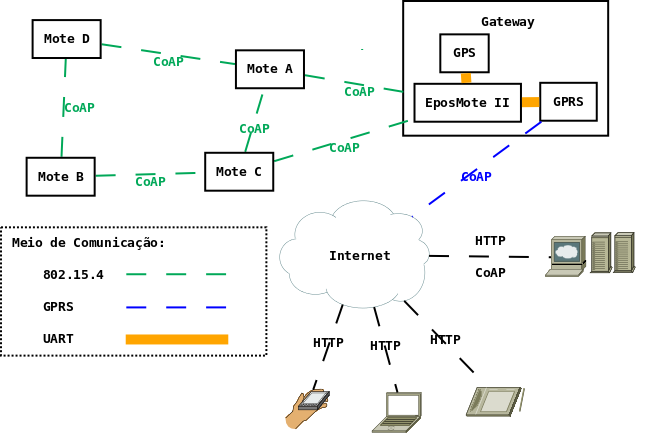
\includegraphics[width=0.8\textwidth]{figuras/arquitetura.png}
   \caption{Vis\~ao geral sobre comunica\c{c}\~ao do sistema.}
\end{figure}

\subsection{Componentes}
O CoAP implementado \'e composto pelos seguintes componentes:



A implementa\c{c}\~ao consiste num m\'odulo que trata requisi\c{c}\~oes, encapsula em pacotes e transmite por mecanimos de transmiss\~ao baseados em \cite{draft-ietf-core-coap-18}.

A biblioteca utilizada para montar o pacote CoAP foi:\\https://github.com/staropram/cantcoap.git. Na qual enviei algumas corre\c{c}\~oes e testes para facilitar a verifica\c{c}\~ao da execu\c{c}\~ao correta dos algoritmos internos durante mudan\c{c}as no c\'odigo. As altera\c{c}\~oes podem ser visualisadas aqui:\\https://github.com/staropram/cantcoap/commits?author=rafaeldelucena.

Para o funcionamento desta biblioteca no EPOS, e para utilizar uma MTU limitada a 128 bytes utilizo um buffer com um valor m\'aximo e armazeno os dados do pacote no buffer. Foi necess\'ario alterar os tipos das vari\'aveis para se adquerem ao EPOS.

O desenvolvimento de um mecanismo de retransmiss\~ao de mensagens n\~ao-confirmadas utilizando uma lista ordenada. Mecanismo de requisic\c{c}\~o e resposta, as requisi\c{c}\~oes pendentes foram armezenadas num Hash com a chave sendo o token gerado pelo cliente.

O protocolo CoAP foi modelado conforme \'e mostrado na figura \ref{uml} abaixo:
\begin{figure}[h]
   \label{uml}
   \centering
   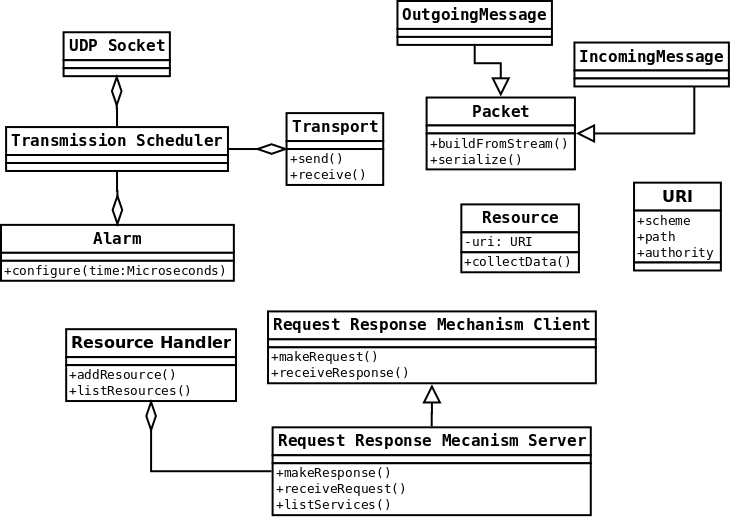
\includegraphics[width=0.9\textwidth]{figuras/uml.png}
   \caption{Diagrama UML das entidades de software implementadas.}
\end{figure}


\begin{figure}[h]
   \label{uml}
   \centering
   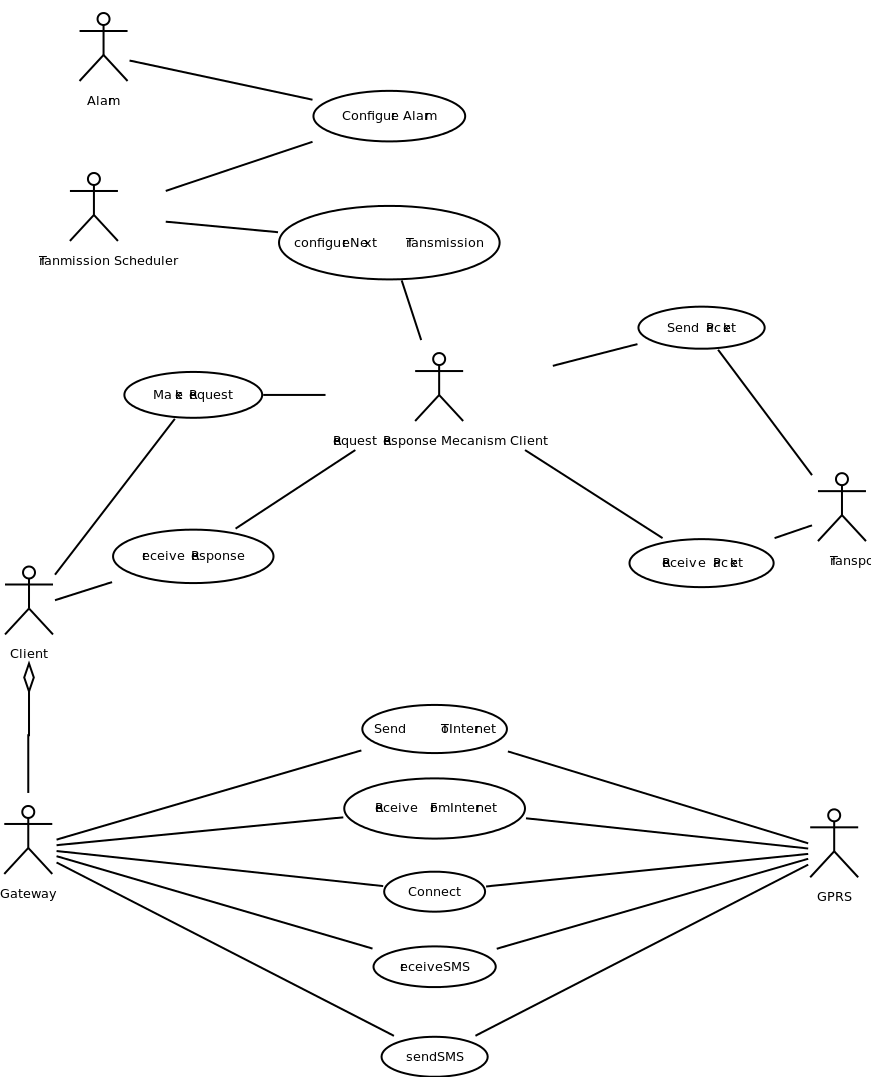
\includegraphics[width=0.8\textwidth]{figuras/casodeuso.png}
   \caption{Diagrama de casos de uso.}
\end{figure}

Para validar o comportamento utilizei alguns testes da pr\'opria biblioteca CoAP portados para o EPOS. Foi necess\'ario implementar a fun\c{c}\~ao assert. J\'a que seria bem mais trabalhoso adicionar uma ferramenta de testes no sistema de build do EPOS.

\section{Testes}
Testes do cliente:
Fazendo uma requisi\c{c}\~ao confirm\'aveis e n\~ao-confirm\'aveis do tipo: GET, POST, PUT, DELETE.
Recebendo respostas: válidas e inválidas.


Testes do Servidor:
Recebendo e respondendo requisi\c{c}\~oes: que possui recurso, que n\~ao possui, descoberta de recurso.

\subsection{Testes na placa de desenvolvimento do m\'ouldo GPRS}
Os testes feitos foram: Enviar e recebimento de mensagens; criar socket TCP, enviar e receber mensagem via socket, fazer requisi\c{c}\~ao HTTP, foi poss\'ivel utilizando os comandos propriet\'arios do modem.


\chapter{Considera\c{c}\~oes Parciais}
O objetivo principal foi atigindo, o desenvolvimento de um gateway simplificado para redes de sensores que utilizem o protocolo CoAP para disponibilizar servi\c{c}os de sensoriamente e atua\c{c}\~ao.

Al\'em disso o consumo de energia e o espa\c{c}os de armazenamento s\~ao muito baixos, respeitando os requis\'itos desse tipo de aplica\c{c}\~ao.

Entres os trabalhos futuros poss\'iveis se destacam os seguintes:
A implementa\c{c}\~ao do protocolo coaps, utilizando DLTS para comunica\c{c}\~ao segura entre os n\'os.

Uma implementa\c{c}\~ao de servidor CoAP completa para executar utilizando a plataforma do EPOSMote II.

Implementa\c{c}\~ao de um gateway que utilize Software Defined Radio, assim apenas um transceiver ser\'a necess\'ario para
fazer a integra\c{c}\~ao com a Internet.

Um gerador de c\'odigo que utiliza como entrada uma linguagem de especifica\c{c}\~ao dos poss\'iveis recursos e como sa\'ida c\'odigo ANSI C m\'inimo de um servidor web utiliza CoAP e seus respectivos recursos. Este gerador deve ser gen\'erico suficiente para ser f\'acil a adapta\c{c}\~ao de diferentes pilhas UDP/IP, arquiteturas e tipos de sensores.


\bibliographystyle{ufscThesis/ufsc-alf}
\bibliography{bibliografia}

%--------------------------------------------------------
% Elementos pós-textuais

\anexo
\chapter{C\'odigo Desenvolvido}
\lstdefinestyle{customc}{
  belowcaptionskip=1\baselineskip,
  breaklines=true,
  xleftmargin=\parindent,
  language=C++,
  showstringspaces=false,
  basicstyle=\scriptsize\ttfamily,
  keywordstyle=\bfseries\color{green!40!black},
  commentstyle=\itshape\color{blue},
  identifierstyle=\color{blue!20!black},
  stringstyle=\color{red},
}

\subsection{CoAP}

\begin{lstlisting}

#ifndef __coap_packet_h__
#define __coap_packet_h__

#include <coap_pdu.h>

__BEGIN_SYS

class CoapPacket : public CoapPDU
{
    public:
        static const int ackTimeout = 2000000;
        static const double ackRandomFactor = 1.5;
        static const int maxRetransmit = 4;
        static const int nStart = 1;

        CoapPacket(const UDP_Address & to);
        CoapPacket(const UDP_Address & from, const char * data, unsigned len);
        CoapPacket(CoapPDU * pdu);
        CoapPacket();
        ~CoapPacket();

        bool isConfirmable();
        bool isConfirmed();
        bool isFailure() {return false;};
        void setConfirmed();
        void reset();
        virtual void update() {kout << "Packet update" << endl;};
        UDP_Address remote() const;
        int getToken();
    protected:
        void generateNewToken(unsigned int len);
    private:
        static const int _maxPDUSize = 100;
        bool _isConfirmed;
        UDP_Address _remote;
        u8 _pduBuffer[_maxPDUSize];
        Alarm * _alarm;
};

class CoapACK : public CoapPacket
{
    public:
        CoapACK(int id) : CoapPacket() {
            setType(CoapPacket::COAP_ACKNOWLEDGEMENT);
            setCode(CoapPacket::COAP_EMPTY);
            setMessageID(id);
        }
};

class CoapConfirmable : public CoapPacket {
    public:
        CoapConfirmable(CoapPacket::Code code);
        ~CoapConfirmable();
        void update();
        bool isFailure();
        void reset();
    private:
        Alarm * _alarm;
        int _retransmissionCounter;
        int _timeout;
};

__END_SYS

#endif /*__coap_packet_h__*/


#ifndef __coap_request_h__
#define __coap_request_h__

#include <coap_packet.h>

__BEGIN_SYS

class CoapRequest : public CoapConfirmable
{
    public:
        CoapRequest(CoapPacket::Code code, const char* uri);
        virtual void onSuccess();
        virtual void onError();
        static void incomingResponse(CoapPacket * packet);
        bool wasAnswered() { return (_response != 0);}
    private:
        void addResponse(CoapPacket *);
        void addAsPending();
        static CoapRequest * removePendingByToken(int token);
        static unsigned int indexByToken(int token);
        static const int _maxPDUSize = 100;
        static const int _maxPending = 100;
        char _uriBuffer[_maxPDUSize];
        int _uriSize;
        static CoapRequest * _pendingRequests[_maxPending];
        CoapPacket * _response;
};

__END_SYS

#endif /*__coap_request_h__*/


#ifndef __coap_response_h__
#define __coap_response_h__

__BEGIN_SYS

class CoapPacket;

template <class T>
class CoapResponse : public CoapPacket
{
    public:
        CoapResponse(T data, CoapRequest * r);
        ~CoapResponse();
    private:
        T * _data;
};

__END_SYS

#endif /*__coap_response_h__*/


#ifndef __coap_socket_h_
#define __coap_socket_h_

#include <udp.h>
#include <coap_packet.h>
#include <utility/queue.h>

#define COAP_PORT 5683

__BEGIN_SYS

class CoapSocket : public UDP::Socket
{
public:
    CoapSocket(const UDP_Address & local);
    ~CoapSocket();
    void sendPacket(CoapPacket * pdu);
    void sendPacket(const CoapPacket & pdu);
    void received(const UDP_Address & from, const char* msg, unsigned int len);
};

__END_SYS

#endif /* __coap_socket_h_ */


#include <coap_packet.h> 
#include <coap_socket.h>
#include <utility/handler.h>
__BEGIN_SYS

class CoapTransport
{
    public:
    static Function_Handler * dispatcher();
    static void incoming(CoapPacket * in);
    static void outgoing(CoapPacket * out);
    
    private:
    CoapTransport();
    ~CoapTransport();
    void addNonConfirmed(CoapPacket* p);
    static void dispatch();
    CoapSocket * _socket;
    Queue<CoapPacket> * _queue;
    Function_Handler * _handler;
    static CoapTransport * getInstance();
    static CoapTransport * _instance;
};
__END_SYS


#include <utility/random.h>
#include <utility/string.h>
#include <coap_packet.h>
#include <coap_transport.h>

__BEGIN_SYS

/*
 * For a new Confirmable message, the initial timeout is set
 * to a random duration (often not an integral number of seconds)
 * between ACK_TIMEOUT and (ACK_TIMEOUT * ACK_RANDOM_FACTOR) (see
 * Section 4.8)
 * */
CoapPacket::CoapPacket(const UDP_Address & to) : CoapPDU(_pduBuffer, _maxPDUSize, 4),
     _remote(to)
{
    setVersion(1);
    _isConfirmed = false;
    int range = (CoapPacket::ackTimeout * CoapPacket::ackRandomFactor) - CoapPacket::ackTimeout;
    int rand = Pseudo_Random::random() % range;
    setMessageID(rand);
}

CoapPacket::CoapPacket() : CoapPDU(_pduBuffer, _maxPDUSize, 4), _remote(UDP_Address("10.0.2.15:5863"))
{
    setVersion(1);
    _isConfirmed = false;
    int range = (CoapPacket::ackTimeout * CoapPacket::ackRandomFactor) - CoapPacket::ackTimeout;
    int rand = Pseudo_Random::random() % range;
    setMessageID(rand);
}

CoapPacket::CoapPacket(const UDP_Address & from, const char * data, unsigned len) : CoapPDU(_pduBuffer, _maxPDUSize, len),
    _remote(from)
{
    strncpy((char*)_pduBuffer, data, len);
}

CoapPacket::CoapPacket(CoapPDU * pdu) : CoapPDU(pdu->getPDUPointer(), _maxPDUSize, pdu->getPDULength()),
    _remote(UDP_Address("10.0.2.15:5863"))
{
    setMessageID(pdu->getMessageID());
}

void CoapPacket::reset()
{
    CoapPDU::reset();
    _isConfirmed = false;
}

int CoapPacket::getToken()
{
    return atol((char*)getTokenPointer());
}

CoapPacket::~CoapPacket()
{
}

CoapConfirmable::~CoapConfirmable()
{
    if (_alarm) delete _alarm;
    _alarm = 0;
}


void CoapConfirmable::reset()
{
    CoapPacket::reset();
    if (_alarm) delete _alarm;
    _alarm = 0;
}

void CoapPacket::setConfirmed()
{
    _isConfirmed = true;
}

bool CoapPacket::isConfirmed()
{
    return _isConfirmed;
}

UDP_Address CoapPacket::remote() const
{
    return _remote;
}

bool CoapPacket::isConfirmable()
{
    return (getType() == CoapPacket::COAP_CONFIRMABLE);
}

void CoapPacket::generateNewToken(unsigned int len)
{
    if (len > 4) return;
    kout << "size of token: " << len << endl;
    int range = 0xFF << len;
    kout << "range:" << range << endl;
    int rand = Pseudo_Random::random() % range;
    kout << "random:" << rand << endl;
    static const int size = 20;
    char buf[size];
    itoa(rand, buf);
    setToken((u8*)buf, len);
}

void CoapConfirmable::update()
{
    kout << "Confirmable update" << endl;
    if (!isConfirmable()) return;
    _retransmissionCounter++;
    _timeout = _timeout * 2;
    if (_alarm) delete _alarm;
    if (isConfirmed()) {
        kout << "already confirmed!" << endl;
        return;
    }
    kout << "configure new alarm with " << _timeout << endl;
    _alarm = new Alarm(_timeout, CoapTransport::dispatcher(), 1);
}

bool CoapConfirmable::isFailure()
{
    return (_retransmissionCounter > CoapPacket::maxRetransmit);
}
        
CoapConfirmable::CoapConfirmable(CoapPacket::Code code) : CoapPacket() {
    setType(CoapPacket::COAP_CONFIRMABLE);
    setCode(code);
    int range = (CoapPacket::ackTimeout * CoapPacket::ackRandomFactor) - CoapPacket::ackTimeout;
    int rand = Pseudo_Random::random() % range;
    _timeout = CoapPacket::ackTimeout + rand;
    _retransmissionCounter = 0;
    _alarm = 0;
}


__END_SYS


#include <system/config.h>
#include <coap_request.h>
#include <coap_transport.h>

__BEGIN_SYS

CoapRequest * CoapRequest::_pendingRequests[] = {0};

CoapRequest::CoapRequest(CoapPacket::Code code, const char* uri)
    : CoapConfirmable(code)
{
    _uriSize = strlen(uri);
    strncpy(_uriBuffer, uri, _uriSize);
    generateNewToken(4);
    setURI(_uriBuffer, _uriSize);
    CoapTransport::outgoing(this);
    addAsPending();
}

void CoapRequest::incomingResponse(CoapPacket * packet)
{
    CoapRequest * req = removePendingByToken(packet->getToken());
    if (req) req->addResponse(packet);
}

void CoapRequest::addResponse(CoapPacket * packet)
{
    if (packet->isFailure()) {
        onError();
    } else {
        onSuccess();
        _response = packet;
    }
}

void CoapRequest::addAsPending()
{
    unsigned int index = indexByToken(getToken());
    CoapRequest::_pendingRequests[index] = this;
}

unsigned int CoapRequest::indexByToken(int token)
{
    return token % CoapRequest::_maxPending;
}

CoapRequest * CoapRequest::removePendingByToken(int token)
{
    unsigned int index = indexByToken(token);
    CoapRequest * ptr = CoapRequest::_pendingRequests[index];
    CoapRequest::_pendingRequests[index] = 0;
    return ptr;
}

void CoapRequest::onSuccess()
{
    kout << "success!" << endl;
}

void CoapRequest::onError()
{
    kout << "error!" << endl;
}

__END_SYS


#include <alarm.h>
#include <utility/handler.h>
#include <utility/list.h>
#include <udp.h>
#include <coap_request.h>
#include <coap_transport.h>

__BEGIN_SYS

static const int idsSize = 1000;
static int ids[idsSize] = {0};

CoapTransport * CoapTransport::_instance = 0; 

static void updateIds(int id) {
    int pos = id % idsSize;
    ids[pos] = id;
}

static bool checkId(int id) {
    int pos = id % idsSize;
    return (ids[pos] == id);
}

CoapTransport * CoapTransport::getInstance()
{
    if (CoapTransport::_instance == 0) {
        CoapTransport::_instance = new CoapTransport();
    }
    return CoapTransport::_instance;
}

CoapTransport::CoapTransport()
{
    _handler = new Function_Handler(CoapTransport::dispatch);
    _queue = new Queue<CoapPacket>();
    _socket = new CoapSocket(UDP_Address(IP::instance()->address(), COAP_PORT));
}

void CoapTransport::dispatch()
{
    CoapTransport * t = CoapTransport::getInstance();
    if (!t) return;
    Queue<CoapPacket>::Element * e = t->_queue->remove();
    CoapPacket * p = e->object();
    if (!p) return;
    if (p->isFailure()){
        kout << "failure "<< endl;
        if (e) delete e;
        return;
    }
    outgoing(p);
    if (e) delete e;
}

void CoapTransport::addNonConfirmed(CoapPacket * p)
{
    Queue<CoapPacket>::Element * e = new Queue<CoapPacket>::Element(p);
    _queue->insert(e);
}

CoapTransport::~CoapTransport()
{
    delete _handler;
    delete _socket;
    delete[] _queue;
}

void CoapTransport::incoming(CoapPacket * in) {
    if (!in) return;
    CoapTransport * t = CoapTransport::getInstance();
    if (!t) return;
    kout << "INCOMING packet" << endl;
    in->print();
    if (in->getType() == CoapPacket::COAP_ACKNOWLEDGEMENT) {
        kout << "is ACK!" << endl;
        updateIds(in->getMessageID());
    }
    if (in->getType() >= CoapPacket::COAP_CREATED) {
        kout << "is a Response!" << endl;
        CoapRequest::incomingResponse(in);
    }
}

void CoapTransport::outgoing(CoapPacket * out)
{
    if (!out) return;
    kout << "OUTGOING packet" << endl;
    kout << "-------------------------" << endl;
    out->print();
    kout << "-------------------------" << endl;
    CoapTransport * t = CoapTransport::getInstance();
    if (!t) return;
    t->_socket->sendPacket(out);
    if (out->isConfirmable()) {
        kout << "Is confirmable!" << endl;
        if (checkId(out->getMessageID())) {
            kout << "is confirmed!" << endl;
            return;
        }
        t->addNonConfirmed(out);
        out->update();
    }
}

Function_Handler * CoapTransport::dispatcher()
{
    CoapTransport * t = CoapTransport::getInstance();
    if (!t) return 0;
    return _instance->_handler;
}

__END_SYS


#include <coap_transport.h>
#include <coap_socket.h>

__BEGIN_SYS

CoapSocket::CoapSocket(const UDP_Address & local) : UDP::Socket(local, UDP::Address(Traits<IP>::BROADCAST, COAP_PORT))
{
}

CoapSocket::~CoapSocket()
{
}

void CoapSocket::received(const UDP_Address& from, const char* data, unsigned int len)
{
	CoapPacket *packet = new CoapPacket(from, data, len);

	if(!packet->validate()) return;
	
	packet->print();

	if (packet->getType() == CoapPacket::COAP_ACKNOWLEDGEMENT) {
	    kout << "is ack!" << endl;
    }

    CoapTransport::incoming(packet);
}

void CoapSocket::sendPacket(CoapPacket * pdu)
{
    if (!pdu) return;
    remote(pdu->remote());
    send(reinterpret_cast<char*>(pdu->getPDUPointer()), pdu->getPDULength());
}

__END_SYS
\end{lstlisting}


\subsection{Aplica\c{c}\~ao WEB}


\end{document}
